% !TeX spellcheck = en_GB
% !TeX root = memoco-report.tex

\section{Dataset generation}
In order to test the two algorithms, a procedure to build a synthetic dataset of different sizes has been provided.\\ 
Given a sequence of holes to be drilled in an electric panel the algorithms should be used to find a sequence of holes that minimizes the cost of drilling the whole panel, where the costs are given by the euclidean distances between holes. For simplicity it is assumed that the cost of drilling every hole can be ignored.\\
The procedure to generate the TSP instances receives as an input a number $N$ of points (which symbolise holes) and generates $N$ pairs representing the coordinates in space of the points on a $N\times N$ square canvas. These points are distributed in a way to resemble the regularity usually found in the disposition of holes in electric panel.\\ 
To do this the procedure draws some regular polygons with up to $10$ sides. Each polygon is generated independently and may overlap with the others, creating not perfectly regular shapes, but neither a completely random point distribution. An example of such an instance is shown in \cref{fig:dataexample}.

\begin{figure}[]
	\centering
	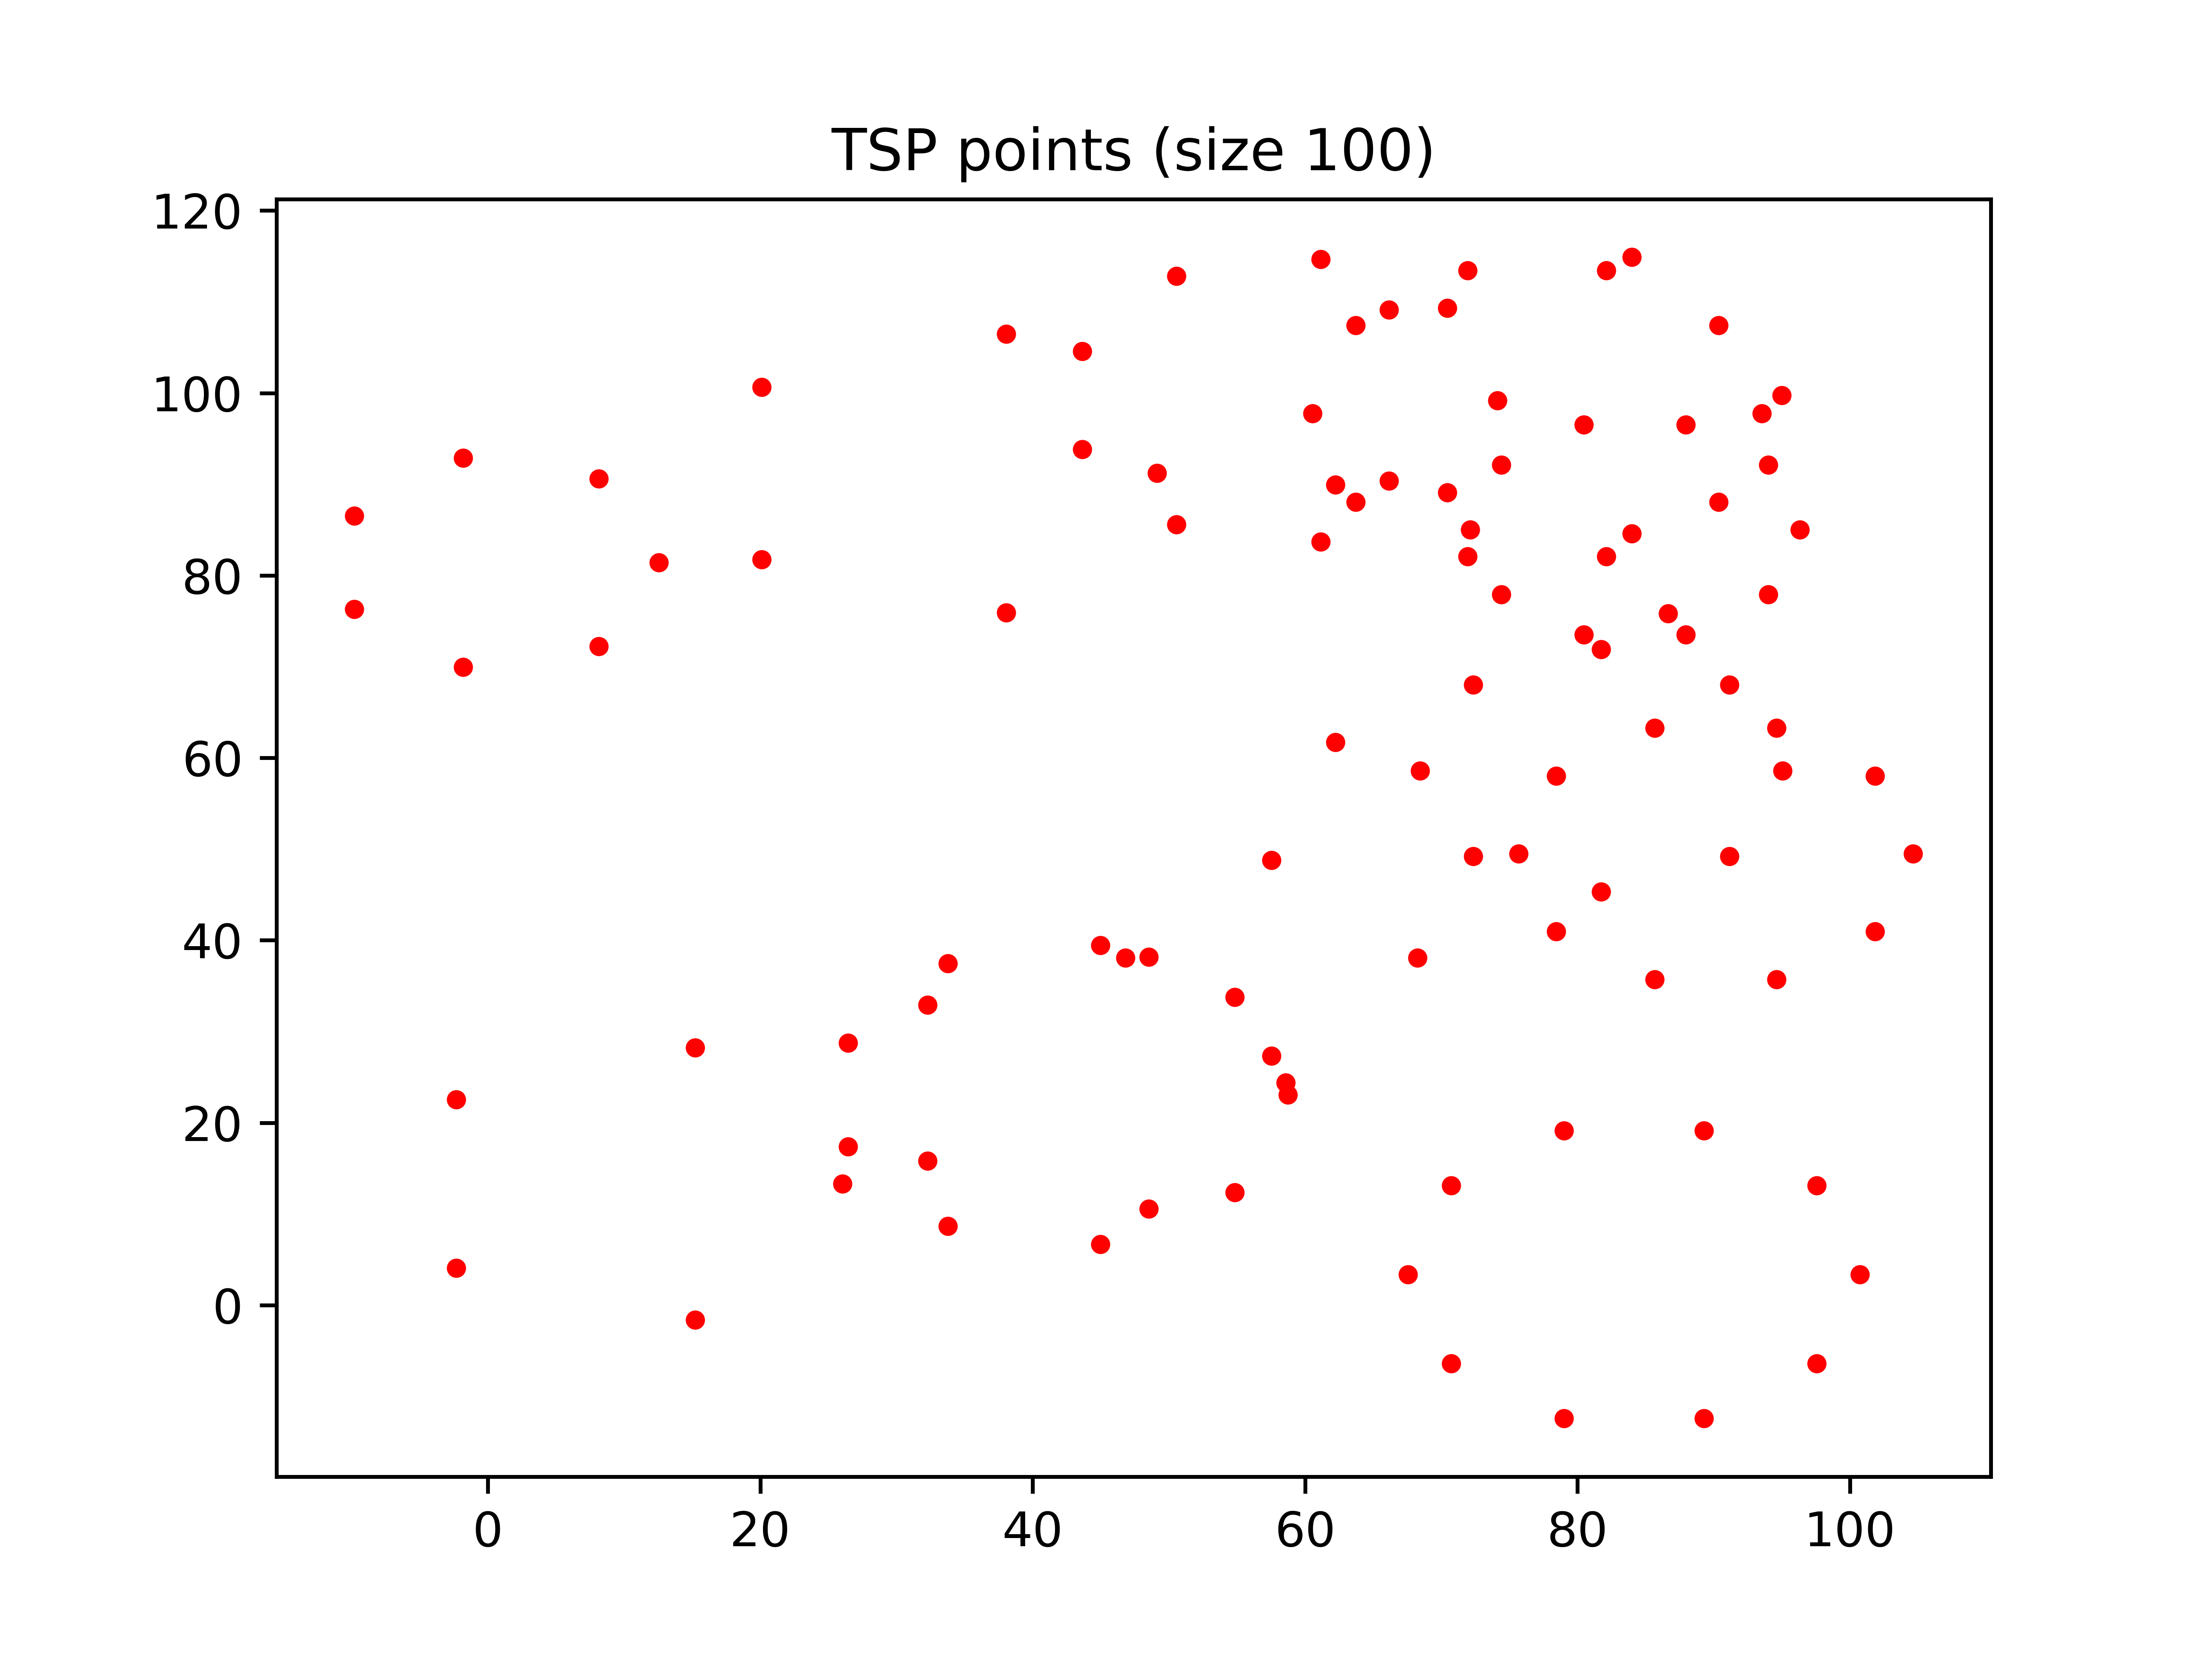
\includegraphics[width=13cm]{path_100}
	\caption{A generated instance of with size N = 100}
	\label{fig:dataexample}
\end{figure}

\section{Exact method}
\label{chap:cplexm}
The exact algorithm makes use of the IBM CPLEX C++ APIs to solve a problem to optimality. In order to model the TSP problem a network flow model is used, as described in the assignment text. \\
The specific linear programming model used and its decision variables are presented below. The set $A$ is the set of edges of the graph, which in this case is a complete graph.
\begin{itemize}
	\item $x_{ij}$ is the amount of 'flow' passed from $i$ to $j,~\forall~(i,j)\in A$
	\item $y_{ij} = 1$ if the edge $(i,j)$ ships some flow, $0$ otherwise $\forall~(i,j)\in A$.
\end{itemize}
\begin{align}
	&\min \sum\limits_{i,j:(i,j)\in A} c_{ij}y_{ij}\\
	&~s.t.~\sum_{i:(i,k)\in A}x_{ik} - \sum_{j:(k,j)\in A, j\ne 0}x_{kj}~~=~1~~~~~~~~~~~~~~~~~~~~~~~\forall~k \in N \setminus \{0\}\\
	& ~~~~~\sum_{j:(i,j)\in A} y_{ij}~~~~~~~~~~~~~~~~~~~~~~~~~~=~1~~~~~~~~~~~~~~~~~~~~~~\forall~i \in N\\
	& ~~~~~\sum_{i:(i,j)\in A} y_{ij}~~~~~~~~~~~~~~~~~~~~~~~~~~=~1~~~~~~~~~~~~~~~~~~~~~~\forall~j \in N\\ 
	&~~~~~~x_{ij}~~~~~~~~~~~~~~~~~~~~~~~~~~~~~~~~~~~\le~(|N|-1)~y_{ij}~~~~~~~\forall~(i,j) \in A,j\ne 0\\
	&~~~~~~x_{ij} \in \mathbb{R}_+~~~~~~~~~~~~~~~~~~~~~~~~~~~~~~~~~~~~~~~~~~~~~~~~~~~~~~~~\forall~(i,j) \in A,j\ne 0\\
	&~~~~~~y_{ij} \in {0,1}~~~~~~~~~~~~~~~~~~~~~~~~~~~~~~~~~~~~~~~~~~~~~~~~~~~~~~~~\forall~(i,j) \in A
\end{align}

The linear programming model is built in the function \texttt{setupLP} in file \texttt{CPLEX.cpp}, and solved calling the IBM CPLEX routines.

\section{Heuristic method}
\label{chap:heuris}

The implemented heuristic is inspired by a popular local search method called Lin-Kernighan heuristic, originally proposed in 1973 in \cite{LinK73}. The algorithm can be considered a generalization of the k-opt algorithm: one of the drawbacks of this algorithm is that the parameter $k$ must be fixed in advance. Instead, the Lin-Kerighan algorithm decides at each iteration, for ascending values of $k$, whether an interchange of $k$ edges provides a better solution. Thus, the algorithm is specified in terms of exchanges (or moves) that can convert one tour into another: given a feasible interchange of $k$ edges (a \textit{k-move}), the algorithm tries to determine if there exists a $k+1$-move that improves the tour further. 
During each iteration, given a feasible tour, the algorithm repeatedly performs exchanges that reduce the length of the current tour, until a tour is reached for which no exchange yields an improvement. This process may be repeated many times from initial tours generated in some possibly randomized way \cite{Helsgaun2000}.\\
So at each iteration the algorithm tries to determine the largest set $X=\{x_1, x_2, ..., x_j\}$ and $Y=\{y_1, y_2, ..., y_j\}$ such that if edges in $X$ (also called the \emph{broken} edges) are removed and replaced by $Y$ (the \emph{joined} edges) the produced tour is a feasible improved (e.g. less costly) solution. Of course, a naive brute force algorithm searching for this sets, would quickly become impractical due to the exponential running time. In order to produce a reasonably efficient local search procedure, the algorithm reduce the search space using the following criteria:
\begin{enumerate}
	\item \emph{Sequential exchange criterion}: each pair of edges $(x_i, y_i)$ and $(y_i, x_{i+1})$ must share one vertex. If $t_1$ and $t_2$ are the vertices of edge $x_1$, then in general for all $i \ge 1$ exchanges are performed this way: $x_i=(t_{2i-1}, t_{2i})$ and $y_i=(t_{2i}, t_{2i+1})$ and $x_{i+1}=(t_{2i+1}, t_{2i+2})$.\\ All \emph{sequential} k-opt moves can be found by concatenating smaller sequential moves, but \emph{non sequential} moves can not be found with this algorithm. An example of such a move is given in \cref{fig:doublebridge}.
	\item \emph{Feasibility criterion}: for every $i \ge 3$, $x_i=(t_{2i-1}, t_{2i})$ is chosen so that if $t_{2i}$ is connected to $t_1$ the resulting configuration is a tour (e.g. a feasible solution). It can be easily seen that at most one choice for $x_i$ satisfies this constraint. Exceptionally, when $i=2$, the originally proposed algorithm allowed for the choice of an $x_i$ which violates this rule. This was done to strengthen the procedure, while not allowing backtracking at every levels significantly reduce running time;
	\item \emph{Positive gain criterion}: let $g_i=cost(x_i) - cost(y_i)$ be the gain by exchanging two edges, and let $G_i=g_1+g_2+...+g_i$ be the partial sum of the gains up to the $i^{th}$ exchange. This criterion requires that each $y_j$ is chosen such that $G_j$ is positive. This choice is justified in \cite{Helsgaun2000};
	\item \emph{Disjunctivity criterion}: sets $X$ and $Y$ must be disjoint.
\end{enumerate}

\begin{figure}[]
	\centering
	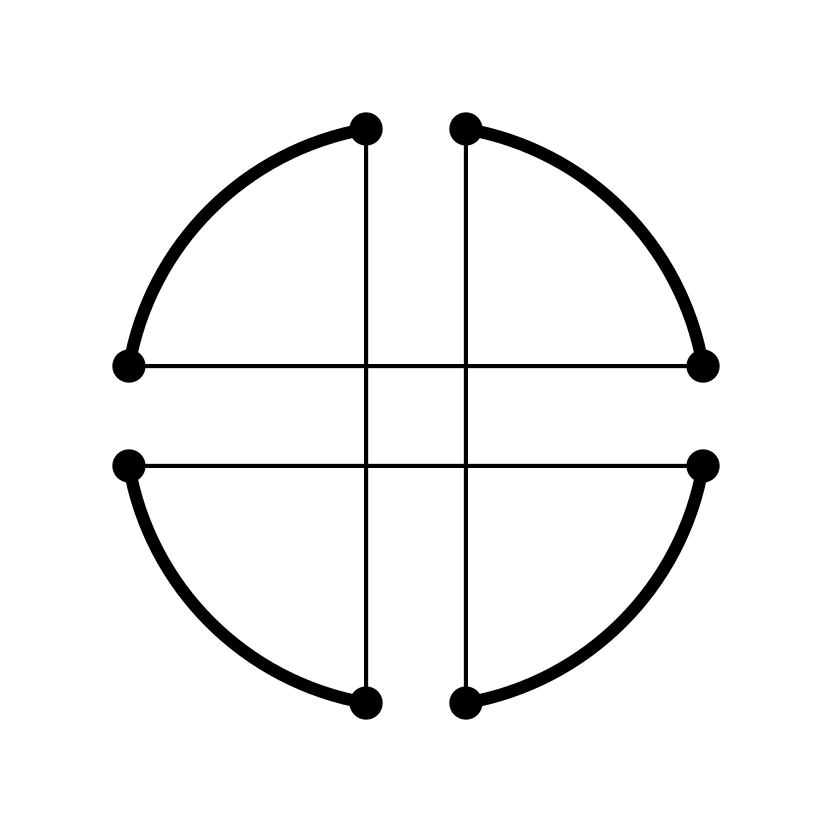
\includegraphics[width=6cm]{double-bridge}
	\caption{A non sequential \emph{double bridge} move with $k=4$}
	\label{fig:doublebridge}
\end{figure}

%\begin{enumerate}
%	\item Start from a (possibly random) feasible solution;
%	\item Choose an initial vertex $s$;
%	\item Remove an edge $x_1 = (s, v)$ which belongs to the current solution and add an edge $y_1 = (v, z)$ ($z \ne s$) which does not belong to the current solution, such that the gain of this move (removal and insertion) is positive;
%	\item Perform step 3 with the following additional constraints:
%	\begin{itemize}
%		\item the edge to remove ($x_i$) must share 1 vertex with the previous added edge ($y_{i-1}$);
%		\item the edge to remove $x_i = (a, b)$ must be chosen such that if $b$ reconnects to the starting vertex $s$ with edge $(b, s)$, the produced solution is feasible;
%		\item the gain (decrease of objective value) of the solution found with previous constraint must be greater than the best increase found so far.
%	\end{itemize}
%	If the second and third conditions are satisfied, the procedure saves this feasible solution, updates the best gain, and proceeds to step 5. Otherwise it tries the other possibility for $x_i$. If this fails too the procedure stops, and the last saved solution is returned;
%	\item Repeat step 4. When no improving solution can be found set the current best solution as starting solution and restart from step 2.
%\end{enumerate}

As reported in \cite{LinK73}, various enhancements are possible. The next sections describe some details and improvement of the implemented algorithm.

\subsection{Stopping criterion}
The algorithm uses the same stopping criterion suggested in the original paper. In particular, when the algorithm finds a feasible tour with a move of size $k$, it checks whether the total gain is the best seen so far. If it is then it is the best improvement seen and it saves the current solution, and tries to improve further with a $k+1$ move. If this doesn't improve the solution the algorithm returns the solution it saved. On the other hand, if the size $k$ move yields a feasible tour which is not the best seen so far, the algorithm stops, since it knows there is a better move, with size smaller than $k$, that produces a better tour.

\subsection{Search intensification}
\label{ssec:intensification}
Between the iterations the algorithm may find some 'good' edges which belongs to the optimal solution or to some reasonably good ones. Subsequently some time may be lost by repeatedly breaking and adding them, while not exploring some more profitable moves. \\
In addition these 'good' edges are likely to be present in many of the best solutions (local optima) found between iterations. In order to direct the search towards more promising solutions, the algorithm keeps track of the edges shared by best $S$ solutions by computing their intersection.\\ 
On the other hand, if the top-S solutions do not include the global optimum, this approach  may prevent the algorithm from breaking some edges which do not belong to the optimum, thus preventing the algorithm from finding it.\\ To mitigate this problem, the intensification procedure is applied only after a specified number of improving moves (i.e. after a fixed $i$). This means that the algorithm has a way to escape this additional constraint for a small number of moves, allowing it to recover from previous sub-optimal choices.\\ 
Additionally, after a local optima is found, the objective value is tested to see if it is better than one of the top-S solutions and in this case the worst solution is replaced with the new one and the intersection is updated.\\
A max-heap data structure is used in order to efficiently replace the worst (i.e. with higher objective value) local optima, and the collection of edges of each tour is maintained in a \texttt{std::set} ordered container, which allows the intersection procedure to take time $O(N\cdot S)$ where $N$ is the number of edges in a feasible tour.\\
In choosing the parameter $S$ it is important to keep in mind that intensification is done only after $S$ local optima are found, so one should ensure that this number is suitable for the problem dimension, because a very large number with a small problem would probably be ineffective.

\subsection{Early stopping}
The authors of the algorithm stated that 30\% to 50\% of running time could be saved by keeping track of previous local optima and stopping the algorithm if the current local optima is the same seen before. This is justified by the fact that if the algorithm couldn't improve this solution before, it's unlikely it can do it now. While this sounds reasonable, in the proposed implementation no particular speed-up was registered. This may be due to the very different computing capabilities of the hardware used in 1973.\\
Since trying to improve a previously found local optima will likely fail, the proposed algorithm adopts a slightly different strategy in this eventuality: instead of stopping, it restarts from a different starting edge and proceeds normally until it finds a different solution, or it determines no better tour exists. While this does not guarantee an improvement in running time, it makes the algorithm redirect the search in a different direction, which is probably more useful that exploring the neighbourhood of a previous solution.\\
To do this, an \texttt{std::set} data structure is used, which maintains a sorted collection (ordered by tour cost) of all the feasible tours found at each iteration. This container guarantees logarithmic insertion and search operations.\\
This strategy could be improved by ensuring that a reasonable number of edges belonging to the previously encountered solution, are not added again.

\subsection{Neighbourhood function}
The algorithm uses a neighbourhood function to determine which move to perform: for a given $i$ a move consists in the selection of an edge $x_i$ to remove and an edge $y_i$ to add to the tour, chosen with the criteria described in \cref{chap:heuris}.
There are exactly two choices for each node to remove (fixing the vertex $t_{2i-1}$), since by the \emph{sequential exchange criterion} $x_i$ must share an endpoint with $y_{i-1}$. Additionally, by the \emph{feasibility criterion}, there is only one choice of $x_i$ that will produce a feasible tour.\\
Starting from vertex $t_{2i-1}$ the algorithm analyses the two possibilities giving the precedence to the most gainful one (the edge with higher cost is the best one to remove). Only if the feasibility criterion is violated the procedure will try to remove the other edge.\\

In order to choose an edge $y_i$, the algorithm finds all possible edges starting in $t_{2i}$ which are 
\begin{itemize}
	\setlength\itemsep{0.05em}
	\item not part of the current solution;
	\item not already broken;
	\item not already joined.
\end{itemize}
In addition for each candidate edge $y_i$, the following two candidates for $x_{i+1}$ are analysed, and the potential gain of adding $y_i$ and removing $x_{i+1}$ is computed. Since the algorithm does not know which choice of $x_{i+1}$ gives the feasible tour, in analysing the two alternatives for $x_{i+1}$, the one with higher cost is considered. So the potential gain is the best possible gain by removing $y_i$ and adding $x_{i+1}$. This score is used to rank the candidates for $y_i$ and is meant to avoid bad choices based on too greedy criteria, like basing the choice only on the cost of the edge to add without any lookahead.

\subsection{Random restart}
The described heuristic is run from a randomized initial solution. Starting from a better solution has been tried, but no significant improvements have been noticed. \\ Since the initial random tour has a significant impact on the heuristic performance ...

\subsection{Hyperparameters}
Table \ref{tab:hyperparameters} includes a description of each parameter to be set in file \texttt{config.yml} before starting the heuristic. Calibration of this hyperparameters are discussed in the next section.

\LTXtable{\linewidth}{parameters}




\subsubsection{Calibration}




%%% Local Variables: 
%%% mode: latex
%%% TeX-master: "isae-report-template"
%%% End: 